\documentclass[handout]{beamer}


\usetheme{default}
\usepackage{subfigure}
\usepackage{amsmath}
\usepackage{Sweave}
\usepackage{graphicx}
\usepackage{color}
\usepackage{multicol}
\usepackage{bm}


\author{Patrick Lam}
\title{Sampling Methods}
\date{}
%\date{October 20, 2008}

\begin{document}

\newcommand{\red}{\textcolor{red}}
\newcommand{\blue}{\textcolor{blue}}
\newcommand{\purple}{\textcolor{purple}}

\frame{\titlepage}

\begin{frame}
\frametitle{Outline}
\tableofcontents
\end{frame}


\section{Inverse CDF Method}

\begin{frame}
\frametitle{Outline}
\tableofcontents[currentsection]
\end{frame}

\begin{frame}
\frametitle{Inverse CDF Method}
\pause
Suppose we want to sample from some \textbf{continuous} distribution
$\blue{f(x)}$, but we only know the CDF $F(x)$ and we are unable to
take derivatives.  \\
\pause
\bigskip
We can sample from $\blue{f(x)}$ if we can sample from a Uniform(0,1)
distribution and know the \textbf{inverse CDF} $F^{-1}(u)$, \pause where
\begin{eqnarray*}
F(x) &=& u\\
F^{-1}(u) &=& x\\
\end{eqnarray*}
\pause
Repeat the following two steps $m$ times:
\pause
\begin{enumerate}
\item Draw a random value from the Uniform(0,1)
distribution. Call this value $u$.
\pause
\item Compute $F^{-1}(u)$ to get a value $x$.  $x$ is a
draw from $\blue{f(x)}$.
\end{enumerate}
\end{frame}

\begin{frame}
\frametitle{An Example}
\pause
Suppose our target density (the one we want to sample from) is the triangle density:
\pause
\begin{eqnarray*}
\blue{f(x) = \left\lbrace \begin{array}{ll} 8x & \mathrm{if} \;
0 \le x < 0.25 \\
\frac{8}{3} - \frac{8}{3} x & \mathrm{if} \; 0.25 \le x \le 1 \\
0 & \mathrm{otherwise} \end{array} \right.}
\end{eqnarray*}
\pause
Now suppose we didn't know $\blue{f(x)}$, but we did know the CDF F(x):
\pause
\begin{eqnarray*}
F(x) &=& \left\lbrace \begin{array}{ll} 0 & \mathrm{if} \; x < 0 \\
4x^2 & \mathrm{if} \; 0 \le x < 0.25 \\
\frac{8}{3}x - \frac{4}{3}x^2 - \frac{1}{3} & \mathrm{if} \; 0.25 \le x \le 1 \\
1 & \mathrm{if} \; x > 1 \\
\end{array} \right.\\
\end{eqnarray*}
\pause
If we stick in a value of $x$ into $F(x)$, we get some value $u$ in
the interval [0,1] (which corresponds to $P(X \le x)$).
\end{frame}

\begin{frame}
Now we need to find $F^{-1}(u)$ such that if we stick in a value of
$u$, we get the corresponding $x$ value.\\
\pause
\bigskip
To do so, we simply set $F(x) = u$ and solve for $x$.
\pause
\begin{eqnarray*}
F^{-1}(u) &=& \left\lbrace \begin{array}{ll} \frac{\sqrt{u}}{2} & \mathrm{if} \; 0 \le u < 0.25 \\
1 - \frac{\sqrt{3(1-u)}}{2} & \mathrm{if} \; 0.25 \le u \le 1 \\
\end{array} \right.\\
\end{eqnarray*}
\pause
For this problem, $F^{-1}(u)$ has a restricted domain of $[0,1]$
because there are no solutions for $u \notin [0,1]$.  Since $u$
is drawn from the Uniform(0,1) distribution, we do not have to worry
about it.\\
\pause
\bigskip
Now we can sample using the inverse cdf method.
\end{frame}

\begin{frame}[fragile]
\begin{enumerate}
\item Draw $m$ random values from the Uniform(0,1) distribution.  Call
these values $\mathbf{u}$.
\pause
\tiny
\medskip
\begin{Schunk}
\begin{Sinput}
> m <- 10000
> u <- runif(m, 0, 1)
\end{Sinput}
\end{Schunk}
\pause
\normalsize
\bigskip
\item Compute $F^{-1}(\mathbf{u})$ to get values of $\mathbf{x}$.  The
values in $\mathbf{x}$ are draws from $\blue{f(x)}$.
\tiny
\pause
\medskip
\begin{Schunk}
\begin{Sinput}
> invcdf.func <- function(u) {
+     if (u >= 0 && u < 0.25) 
+         sqrt(u)/2
+     else if (u >= 0.25 && u <= 1) 
+         1 - sqrt(3 * (1 - u))/2
+ }
> x <- unlist(lapply(u, invcdf.func))
\end{Sinput}
\end{Schunk}
\end{enumerate}
\end{frame}

\begin{frame}[fragile]
We can compare the density of our draws to the target density $\blue{f(x)}$.
\pause
\begin{figure}
\begin{center}
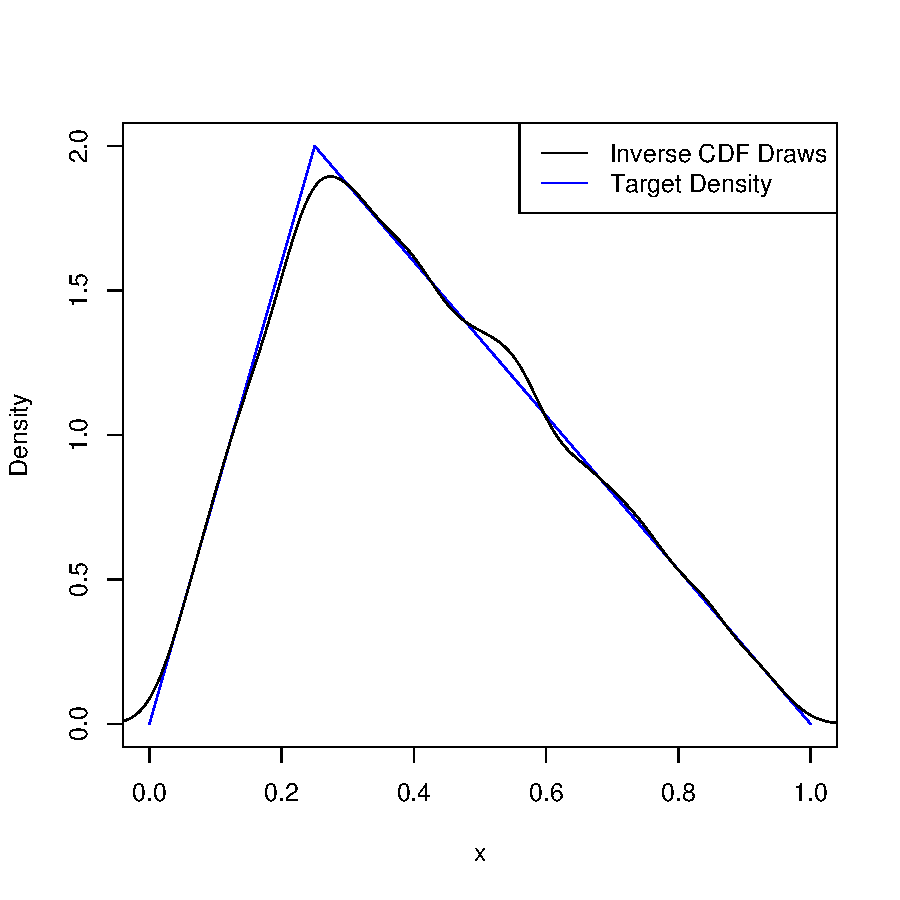
\includegraphics[width = 2.5in, height = 2.5in]{sampling-invcdf.pdf}
\end{center}
\end{figure} 
\end{frame}

\begin{frame}
\frametitle{Why Does It Work?}
\pause
\begin{figure}[!htp]
\begin{center}
\subfigure{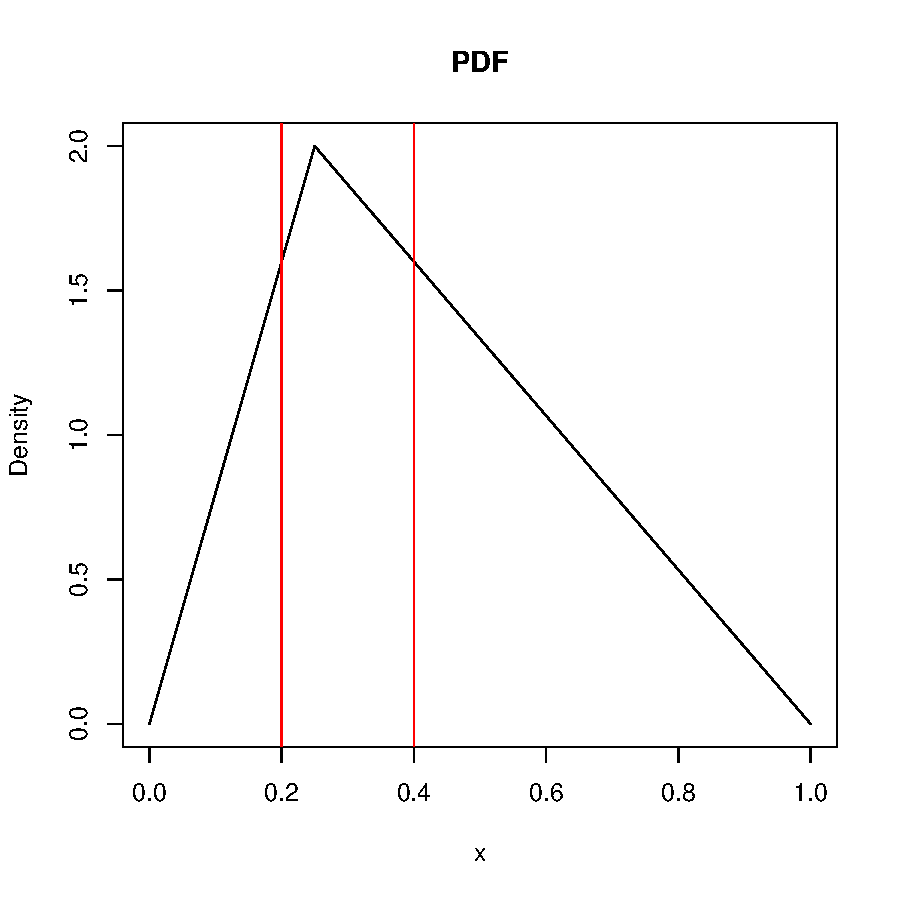
\includegraphics[width = 2in, height = 2in]{sampling-tripdf.pdf}}
\subfigure{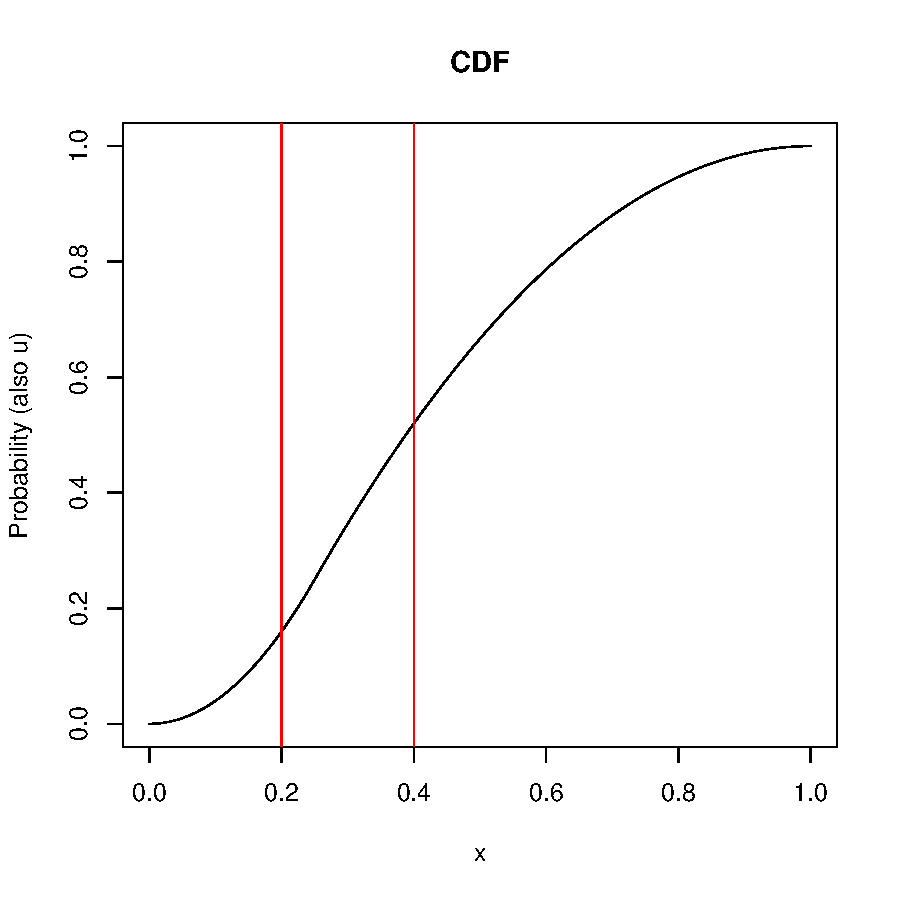
\includegraphics[width = 2in, height = 2in]{sampling-tricdf.pdf}} 
\end{center}
\end{figure}
\pause
The areas with more density on the PDF (for example, the interval [0.2,0.4])
have a steeper ``slope'' on the CDF, so they cover more of the [0,1]
space of $u$, and thus will be drawn more often.
\end{frame}

\section{Rejection Sampling}

\begin{frame}
\frametitle{Outline}
\tableofcontents[currentsection]
\end{frame}

\begin{frame}
\frametitle{Rejection Sampling}
\pause
Suppose again that we want to sample from our target density
$\blue{f(x)}$, which in our example is the triangle density.\\
\pause
\bigskip
For the rejection sampling, we need to pick a candidate density
$\purple{g(x)}$ such that $\blue{f(x)} \le M\purple{g(x)}$ for all
$x$, where $M$ is a constant.\\
\pause
\bigskip
Repeat the following steps until we get $m$ accepted draws:
\pause
\begin{enumerate}
\item Draw a candidate $x_c$ from $\purple{g(x)}$.  
\pause
\item Calculate an acceptance probability $\alpha$ for $x_c$.
\pause
\begin{eqnarray*}
\alpha = \frac{\blue{f(x_c)}}{M \purple{g(x_c)}}
\end{eqnarray*}
\pause
\item Draw a value $u$ from the Uniform(0,1) distribution.
\pause
\item Accept $x_c$ as a draw from $\blue{f(x)}$ if $\alpha \ge u$.
Otherwise, reject $x_c$ and go back to step 1.
\end{enumerate}

\end{frame}

\begin{frame}[fragile]
\frametitle{An Example}
\pause
Target Density $\blue{f(x)}$ (the triangle density):
\pause
\medskip
\tiny
\begin{Schunk}
\begin{Sinput}
> f.x <- function(x) {
+     if (x >= 0 && x < 0.25) 
+         8 * x
+     else if (x >= 0.25 && x <= 1) 
+         8/3 - 8 * x/3
+     else 0
+ }
\end{Sinput}
\end{Schunk}
\pause
\normalsize
\bigskip
For our candidate density $\purple{g(x)}$, let's use the Uniform(0,1) density:
\pause
\medskip
\tiny
\begin{Schunk}
\begin{Sinput}
> g.x <- function(x) {
+     if (x >= 0 && x <= 1) 
+         1
+     else 0
+ }
\end{Sinput}
\end{Schunk}
\pause
\bigskip
\normalsize
Let's set $M = 3$ because I know from guess and check that
$\blue{f(x)}$ is never greater than $M \purple{g(x)}$, which is 3 for all
$x \in [0,1]$.
\tiny
\medskip
\pause
\begin{Schunk}
\begin{Sinput}
> M <- 3
\end{Sinput}
\end{Schunk}
\normalsize
\end{frame}

\begin{frame}
\begin{figure}[!htp]
\begin{center}
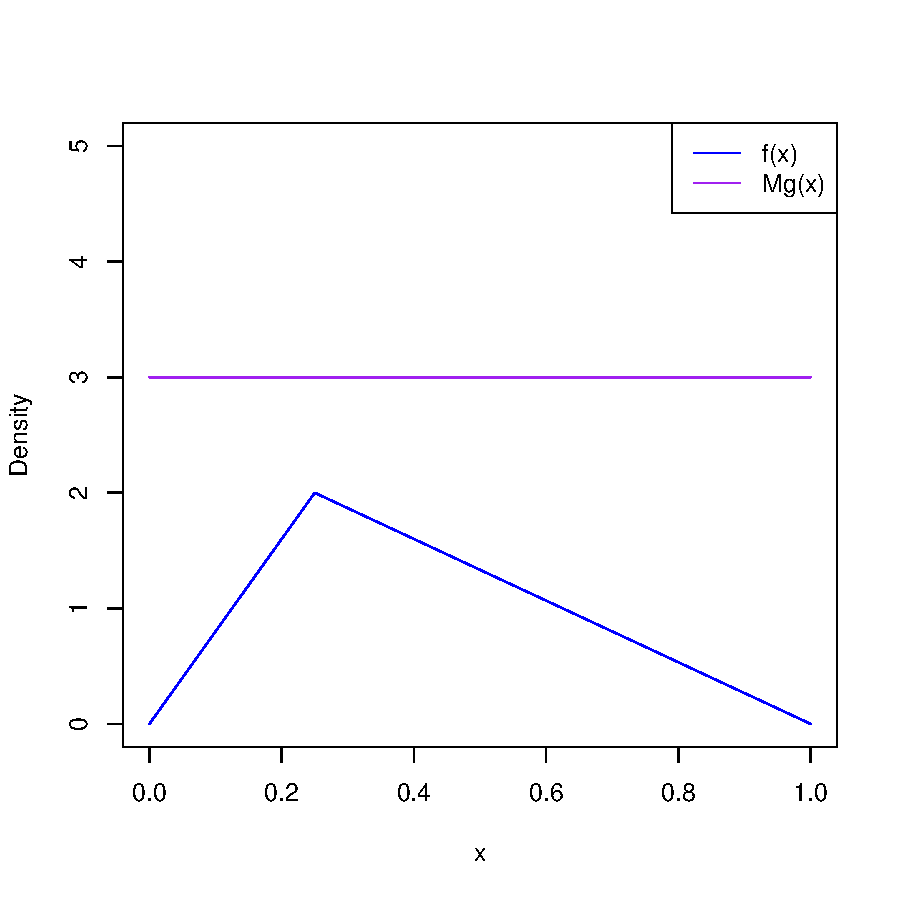
\includegraphics[width = 3in, height = 3in]{sampling-triunif.pdf}
\end{center}
\end{figure}
\end{frame}

\begin{frame}[fragile]
Let's do rejection sampling!
\pause
\begin{enumerate}
\item Draw a candidate $x_c$ from $\purple{g(x)}$.  
\pause
\item Calculate an acceptance probability $\alpha =
\frac{\blue{f(x_c)}}{M \purple{g(x_c)}}$ for $x_c$.
\pause
\item Draw a value $u$ from the Uniform(0,1) distribution.
\pause
\item Accept $x_c$ as a draw from $\blue{f(x)}$ if $\alpha \ge u$.
Otherwise, reject $x_c$ and go back to step 1.
\end{enumerate}
\tiny
\pause
\medskip
\begin{Schunk}
\begin{Sinput}
> m <- 10000
> n.draws <- 0
> draws <- c()
> x.grid <- seq(0, 1, by = 0.01)
> while (n.draws < m) {
+     x.c <- runif(1, 0, 1)
+     accept.prob <- f.x(x.c)/(M * g.x(x.c))
+     u <- runif(1, 0, 1)
+     if (accept.prob >= u) {
+         draws <- c(draws, x.c)
+         n.draws <- n.draws + 1
+     }
+ }
\end{Sinput}
\end{Schunk}
\end{frame}

\begin{frame}
\begin{figure}[!htp]
\begin{center}
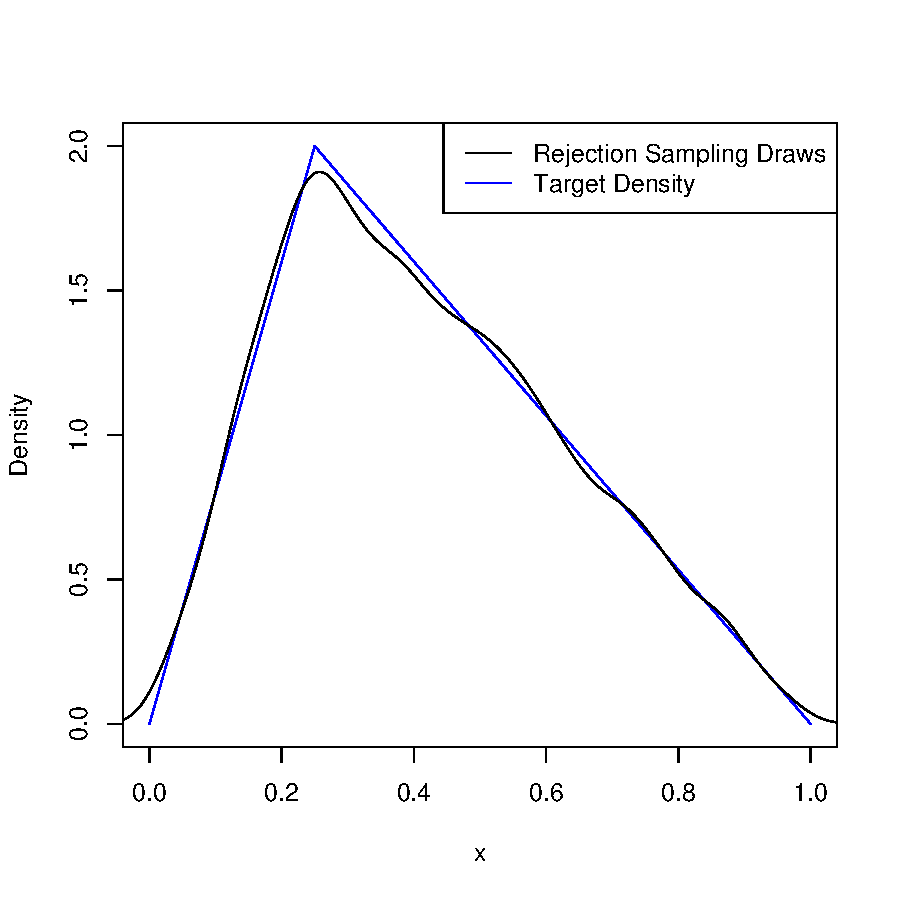
\includegraphics[width = 3in, height = 3in]{sampling-reject1.pdf}
\end{center}
\end{figure}
\end{frame}

\begin{frame}
\frametitle{Why Does It Work?}
\pause
\begin{figure}[!htp]
\begin{center}
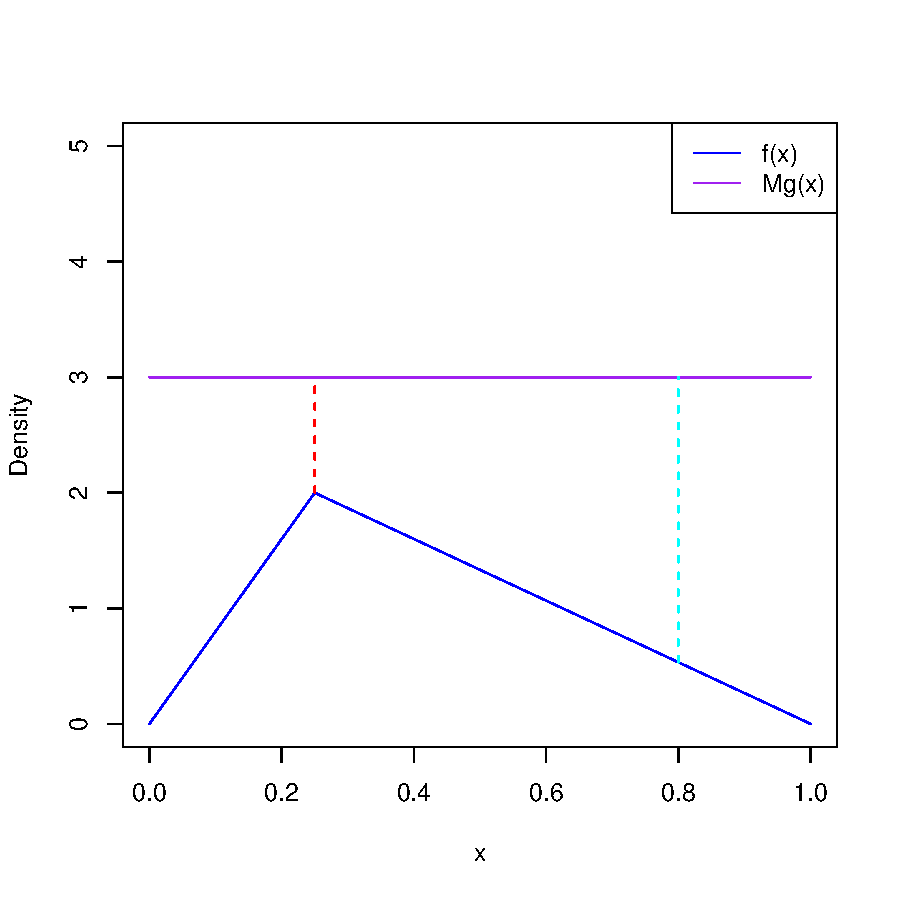
\includegraphics[width = 2in, height = 2in]{sampling-triunif2.pdf}
\end{center}
\end{figure}
\pause
The difference between $\blue{f(x)}$ and $M\purple{g(x)}$ at places
with higher density (i.e. around \red{$x = 0.25$}) is smaller than at
places with lower density (i.e. around \textcolor{cyan}{$x = 0.8$}),
\pause so the acceptance probability at \red{$x = 0.25$} is higher and
\pause more draws of \red{$x = 0.25$} are accepted.
\end{frame}

\begin{frame}
There are an infinite number of candidate densities $\purple{g(x)}$
and constants M that we can use.\\
\pause
\bigskip
The only difference between them is computation time.\\
\pause
\bigskip
If $\purple{g(x)}$ is significantly different in shape than
$\blue{f(x)}$ or if $M \purple{g(x)}$ is significantly greater than
$\blue{f(x)}$, then more of our candidate draws will be rejected. \\
\pause
\bigskip
If $\blue{f(x)} = M \purple{g(x)}$, then all our draws will be accepted.\\
\pause
\bigskip
A version of rejection sampling forms the basis for the
Metropolis-Hastings algorithm that we will use later to sample from
(possibly multivariate) posteriors without knowing the normalizing constant.
\end{frame}
\end{document}
